\documentclass[10pt]{beamer}
\setbeamertemplate{bibliography item}[triangle]

\usetheme{metropolis}
\usepackage{appendixnumberbeamer}

\usepackage{booktabs}
\usepackage[scale=2]{ccicons}

\usepackage{pgfplots}
\usepgfplotslibrary{dateplot}
\newcommand{\ra}{\rightarrow}
\newcommand{\la}{\leftarrow}
\newcommand{\ua}{\uparrow}
\newcommand{\da}{\downarrow}
\renewcommand{\S}{\mathcal{S}}
\newcommand{\A}{\mathcal{A}}
\newcommand{\E}{\mathbf{E}}
\newcommand{\U}{\mathcal{U}}
\newcommand{\R}{\mathbb{R}}
\newcommand{\eqdef}{\stackrel{\cdot}{=}}
\newcommand{\tu}{\tilde{u}}
\newcommand{\tj}{\tilde{J}}
\newcommand{\tr}{\tilde{r}}
\newcommand{\minp}{(\min,+)}
\newcommand{\op}{\oplus}
\newcommand{\om}{\otimes}
\newcommand{\V}{\mathcal{V}}
\newcommand{\mb}{\mbox{ }}
\newcommand{\norm}[1]{\|#1\|}
\newcommand{\inorm}[1]{\|#1\|_{\infty}}
\newcommand{\snorm}[1]{\left\|#1\right\|}
\newcommand{\sinorm}[1]{\left\|#1\right\|_{\infty}}

\usepackage{caption}
\usepackage{subcaption}
\usepackage{pifont}

\usepackage{xspace}
\newcommand{\themename}{\textbf{\textsc{metropolis}}\xspace}

\title{Sequential Decision Making Under Uncertainty}
%\subtitle{APU}
\date{\today}
\author{Chandrashekar Lakshminarayanan}
\institute{Reinforcement Learning \& Artificial Intelligence Group,\\University of Alberta}
% \titlegraphic{\hfill\includegraphics[height=1.5cm]{logo.pdf}}

\begin{document}

\maketitle
%\begin{frame}{Overview}
%  \setbeamertemplate{section in toc}[sections numbeorange]
%  \tableofcontents[hideallsubsections]
%\end{frame}

\begin{frame}{Overview}
\begin{itemize}
\item {Professional Background and Research Contributions}
\item {Background: Exact \& Approximate Dynamic Programming (ADP) }
\begin{itemize}
\item Issues with State-of-the-Art
\item Gaps
\end{itemize}
\item {Research Contributions}
\begin{itemize}
\item ADP in Tropical Algebra
\item Approximate Linear Programming for Large Scale MDPs: Geometric insights
\end{itemize}
\end{itemize}

\end{frame}



\section{Professional Background and Research Contributions}

\begin{frame}[fragile]{Professional Background}
\begin{itemize}
\item {\color{orange}{Bachelor of Technology}}, with specialization in Instrumentation and Control, from National Institute of Technology, Trichy (2001-2005)
\item {\color{orange}{Analog Design Engineer}}, with specialization in design of high speed Analog to Digital Converters, at Cosmic Circuits Pvt Ltd, Bangalore (2005-2008)
\item {\color{orange}{Master of Engineering}}, with specialization in Systems Science and Automation (SSA), from Indian Institute of Science, Bangalore (2008-2010)
\item {\color{orange}{PhD}}, with specialization in Approximate Dynamic Programming and Reinforcement Learning, from Indian Institute of Science, Bangalore (2010-2015)
\item {\color{orange}{Post Doctoral Fellow }}, in the Reinforcement Learning \& Artificial Intelligence group at the University of Alberta, Canada
\end{itemize}
\end{frame}

\begin{frame}[fragile]{Sequential Decisions under Uncertainty: Example}
\begin{tikzpicture}[overlay]
\node[black] at (7.5,0) {\includegraphics[scale=0.25]{mouse-axes.png}};
\end{tikzpicture}
\color{black}
\begin{block}{Assume}
\begin{itemize}
\item Mouse needs cheese
\item can sense position $(x,y)$
\item Uncertainty to random displacements
\end{itemize}
\end{block}
\begin{block}{Need}
\begin{itemize}
\item Map $u^*: state=(x,y)\ra action=\{Right,Left,Up,Down\}$ for all states
\item Sequence: $state_1-action_1-state_2-action_2,\ldots$
\end{itemize}
\end{block}

\end{frame}



\begin{frame}[fragile]{Sequential Decisions under Uncertainty: Complex Systems}

$\mbox{ }$
\includegraphics[scale=0.125]{atari.jpg}
$\mbox{ }$
\includegraphics[scale=0.125]{queues1.jpg}
$\mbox{ }$
\includegraphics[scale=0.125]{robosoc.jpg}
$\mbox{ }$$\mbox{ }$
\includegraphics[scale=0.125]{invent.jpeg}
$\mbox{ }$\\
$\mbox{ }$
\quad Atari\quad\quad\quad\quad
$\mbox{ }$
Queues\quad\quad\quad\quad
$\mbox{ }$
 Robosoccer\quad\quad
$\mbox{ }$
Inventory
$\mbox{ }$\\
\quad\quad\quad\quad\quad\quad\quad
\quad\quad\quad\quad\quad\quad\quad
\quad\quad\quad\quad\quad\quad\quad
\quad\quad\quad
Control

\begin{figure}
\begin{table}
\begin{tabular}{cc}
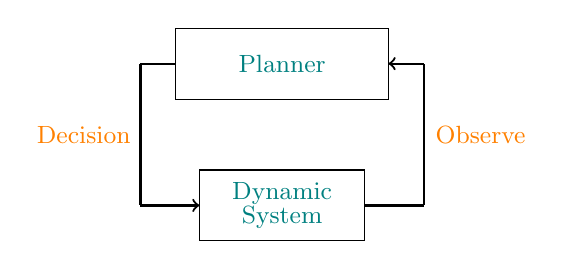
\begin{tikzpicture}[scale=0.6,font=\small,axis/.style={very thick, ->, >=sorangeth'}]

\draw [black=100](-2.25,-1.25) rectangle (2.25,0.25);
\node[teal] at(0,-0.5) {Planner};
%\node[black] at(0,-0.75) {};

\draw [black=100](-1.75,-4.25) rectangle (1.75,-2.75);
\node[teal] at(0,-3.25) {Dynamic};
\node[teal] at(0,-3.75) {System};

\node[orange] at(4.2,-2){\color{orange}{Observe}};


\node[orange] at(-4.2,-2){Decision};

\draw[thick,-](-2.25,-0.5)--(-3,-0.5);
\draw[thick,-](-3,-0.5)--(-3,-3.5);
\draw[thick,->](-3,-3.5)--(-1.75,-3.5);

\draw[thick,->](3,-0.5)--(2.25,-0.5);
\draw[thick,-](3,-3.5)--(3,-0.5);
\draw[thick,-](1.75,-3.5)--(3,-3.5);

\end{tikzpicture}
&
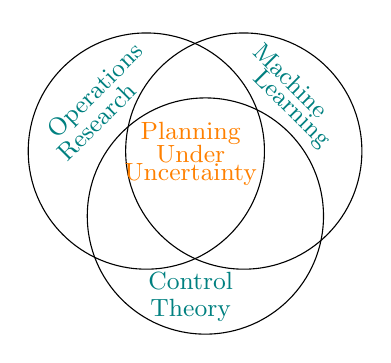
\begin{tikzpicture}[scale=0.75,font=\small,axis/.style={very thick, ->}]
\draw [] (0.9,0.5) circle (2);
\draw [] (-0.75,0.5) circle (2);
\draw [] (.25,-0.6) circle (2);
%\draw [] (-0.5,0.5) circle (2);
%\draw [] (0.5,-0.5) circle (2);
%\draw [] (-0.5,-0.5) circle (2);

\node[orange] at(0,0.8){Planning};

\node[orange] at(0,0.45){Under};
\node[orange] at(0,0.1){Uncertainty};

\node[teal,rotate=-45] at(1.7,1.7){Machine};
\node[teal,rotate=-45] at(1.7,1.2){Learning};

\node[teal,rotate=45] at(-1.6,1.5){Operations};
\node[teal,rotate=45] at(-1.6,1.0){Research};

\node[teal] at(-0,-1.7){Control};
\node[teal] at(-0,-2.2){Theory};
\end{tikzpicture}

\end{tabular}

\end{table}
%\caption*{No Explicit Labels; Control via Feedback }
\end{figure}

\end{frame}

\begin{frame}[fragile]{Overall Scheme and Challenges}

\begin{block}{}
\centering    Model
\end{block}
\centering $\downarrow$
\begin{block}{}
\centering Optimization Problem $(*)$
\end{block}
\centering $\downarrow$
\begin{block}{}
\centering Algorithm to solve $(*)$
\end{block}
\begin{table}
\begin{tabular}{lr}
\begin{minipage}{0.5\textwidth}
\begin{center}
\begin{block}{\centering Roadblock I}
\centering Scale of the System
\end{block}
\end{center}
{\color{orange}{Approximate Algorithms} }
\end{minipage}
&
\begin{minipage}{0.5\textwidth}
\begin{center}
\begin{block}{\centering Roadblock II}
\centering Lack of Model
\end{block}
\end{center}
{\color{orange}{Stochastic Algorithms}}
\end{minipage}


\end{tabular}
\end{table}

\end{frame}


\begin{frame}[fragile]{Research Contributions}
\begin{itemize}
\item {\color{teal}{Convergent approximate algorithms in }} {\color{orange}{tropical linear}} {\color{teal}{basis}}
\item {\color{teal}{Geometric characterization of}} {\color{orange}{approximate linear programming}} {\color{teal}{for large scale Markov Decision Processes}}
\item {\color{teal} {Conditions that imply}} {\color{orange}{stability of multi-timescale stochastic }} {\color{teal}{approximation algorithms}}
\item {\color{teal}{Optimal Pricing of}} {\color{orange}{crowdsourced}} {\color{teal}{tasks}}
\end{itemize}
\end{frame}

\begin{frame}[fragile]{Publications}
\small
\begin{itemize}
\item Chandrashekar, L.; Bhatnagar, S., ``Approximate Dynamic Programming with $(\min,+)$ linear function approximation for Markov Decision Processes," $53^{rd}$ IEEE CDC, 2014\\
\item Chandrashekar, L.; Bhatnagar, S., ``A Generalized Reduced Linear Program for Markov Decision Processes," $29^{th}$ AAAI conference, 2015

\item Chandrashekar, L. and  Bhatnagar, S. ``A Stability Criterion for Two Timescale Stochastic Approximation Schemes",  Automatica, 2017

\item Chandrashekar, L.;  Dubey, A.; Bhatnagar, S. and Chithralekha, B., ``A Markov Decision Process framework for predictable job completion times on crowdsourcing platforms", Proceedings of the Second {AAAI} Conference on Human Computation and Crowdsourcing, {HCOMP} 2014, Pittsburgh, Nov. 2-4, 2014
\item Maity, R. K.; Chandrashekar, L.;  Padakandla, S.; Bhatnagar, S., `` Shaping Proto-Value Functions Using Rewards", European Conference on Artificial Intelligence 2016\\
\item Chandrashekar, L.;  Bhatnagar, S and Szepesv\'{a}ri C., ``A Linearly Reduced Approximate Linear Program for Markov Decision Processes", submitted to IEEE Transactions on Automatic Control
\end{itemize}
\end{frame}



\section{Background: Approximate Dynamic Programming}

\begin{frame}[fragile]{Markov Decision Process (MDP)}
\begin{block}{MDP $\M=<\S,\A,P,g,\alpha>$}
\begin{itemize}
\item State space $\S=\{s^1,\ldots,s^n\}$
\item Action space $\A=\{a^1,\ldots,a^d\}$
\item Markovian Transition
\begin{align*}
Pr\{s_{t+1}=s'| s_t=s, a_t=a\}=p_a(s,s')
\end{align*}
\item Rewards $g_a(s)$ for action $a$ in state $s$
\item Policy: $u\colon \S\ra \A$ (induces a Markov chain with kernel $P_u$)
\item Value: $J_u(s)\eqdef \E\big[\sum_{t=0}^\infty \alpha^t g_{a_t}(s_t)|s_0=s,a_t=u(s_t)\big]$
\end{itemize}
\end{block}
\begin{block}{Aim for optimal}
Compute  $J^*(s)=\max_{u} J(s),\,\forall s\in \S$ and $u^*$ s.t $J_{u^*}=J^*$
\end{block}
\begin{tikzpicture}[overlay]
\node[black] at (10,5) {\includegraphics[scale=0.25]{mouse-single.png}};
\end{tikzpicture}
\end{frame}

\begin{frame}[fragile]{Dynamic Programming}

\begin{block}{Greedy Principle}
{\color{orange}{Best = Current Best+ Future Best}}
\end{block}
\begin{block}{Bellman Equation}
\begin{align*}
J^*(s)&=\alert<3-4>{\max_{a\in \A}} \alert<1>{g_a(s)}+\alert<2>{\alpha p_a(s,\cdot)^\top J^*}\\
\end{align*}
\end{block}
\p\p\p
\vspace{-20pt}
\vspace{-20pt}
\normalsize
\begin{block}{Values lead to Policy}
\begin{align*}
u^*(s)\eqdef \U(J^*)(s) =\alert<4>{\arg\max_{a\in \A}} (g_a(s)+\alpha p_a(s,\cdot)^\top J^*)
\end{align*}
\end{block}
\normalsize
\p
\begin{block}{Bellman Operator}
\begin{align*}
(TJ)(s)&\eqdef\max_{a\in \A} g_a(s)+\alpha p_a(s,\cdot)^\top J
\end{align*}
\end{block}
\normalsize

\end{frame}

\begin{frame}[fragile]{DP Algorithms}
\begin{block}{Value Iteration}
\begin{center}

Power Method: $J_{t+1}=T J_t$
\end{center}
\end{block}
\normalsize\p
\begin{block}{Policy Iteration}

\begin{center}
Evaluation: $J_{u_t}=T_{u_t} J_{u_t}$\\
Improvement: $u_{t+1}=\U J_{u_t}$
\end{center}
\end{block}
\normalsize\p
\begin{block}{Linear Programming}

\begin{align*}
J^*&=\arg\min_{J\in \R^{\S}} c^\top J\\
&\quad s.t. J\geq TJ
\end{align*}
\end{block}
\begin{block}{\centering $L_\infty$ Contraction $\Rightarrow$ Convergence}
\centering {\color{orange}{$\norm{TJ_1-TJ_2}_\infty\leq \alpha \norm{J_1-J_2}_\infty$}}
\end{block}

\end{frame}

\begin{frame}[fragile]{Toy Grid World}

\begin{table}
\begin{tabular}{|c|c|c|}\hline
$\mb $&$\uparrow$	&$G$\\\hline
${\leftarrow}$	&$s$	&$\ra$\\\hline
$\mb$	&$\downarrow$	&$\mb$	\\\hline
\end{tabular}
\end{table}
\begin{itemize}
\item $S=X\times Y$, $A=\{\leftarrow,\rightarrow,\uparrow,\downarrow\}$, $\alpha=0.9$.
\item With $p=0.9$ move to desired position.
\item Reward at $G$ is $1$ otherwise $0$.
\end{itemize}

\begin{table}
\begin{tabular}{|c|c|c|}\hline
~$0$~	&~$0$~	&~$1$~\\\hline
$0$	&$0$	&$0$\\\hline
$0$ &$0$	&$0$\\\hline
\end{tabular}
\begin{tabular}{|c|c|c|}\hline
$0$	&$0.81$	&$1$\\\hline
$0$	&$0$	&$0.81$\\\hline
$0$ &$0$	&$0$\\\hline
\end{tabular}
\end{table}

\begin{table}
\begin{tabular}{|c|c|c|}\hline
$0.72$	&$1.53$	&$1.9$\\\hline
$0$	&$0.72$	&$1.53$\\\hline
$0$      &$0$	&$0.72$\\\hline
\end{tabular}
\begin{tabular}{|c|c|c|}\hline
$7.2$	&$8.1$	&$10$\\\hline
$6.56$	&$7.29$	&$8.1$\\\hline
$5.90$ &$6.56$	&$7.29$\\\hline
\end{tabular}
\end{table}
\begin{tikzpicture}[overlay]
\node[orange] at (4,4.25) {$TJ$};
\node[orange] at (6,4.25) {$T^2J$};

\node[orange] at (4,2.2) {$T^3J$};
\node[orange] at (6,2.2) {$J^*$};

\end{tikzpicture}
\end{frame}



\begin{frame}[fragile]{Exact DP Algorithms }

\begin{algorithm}[H]
\caption*{Template of Exact DP Algorithm}
\begin{algorithmic}[1]
\STATE{Input: Model {\color{orange}{$\M=<\S,\A,P,g,\alpha>$}}}
\STATE{$Exact\, DP(\M)$\{}
\STATE{{\color{orange}{Value/Policy-Iteration, Linear Programming}}}
\STATE{\}}
\STATE{Output: {\color{orange}{ $J^*$}}}
\end{algorithmic}
%\label{mab1}
\end{algorithm}

\begin{itemize}
\item $poly(|\S|,|\A|)$
\item $|\S|$ can blow up exponentially. Example: Queuing system with
    \begin{itemize}
    \item $n$ parallel queues and buffer size $K$
    \item $K^n$ possible configurations
    \end{itemize}
\end{itemize}
\end{frame}



\begin{frame}[fragile]{Handling the Curse of Dimensionality}

\begin{block}{}
\centering    Model (MDP)
\end{block}
\centering $\downarrow$
\begin{block}{}
\centering BE
\end{block}
\centering $\downarrow$
\begin{block}{}
\centering DP Algorithms to solve BE
\end{block}
\begin{block}{\centering Roadblock I}
\centering Scale of the System
\end{block}

{\color{orange}{Approximate Dynamic Programming} }

\end{frame}




\begin{frame}[fragile]{Approximate DP Algorithms}

\begin{algorithm}[H]
\caption*{Template of Approximate DP Algorithm}
\begin{algorithmic}[1]
\STATE{Input: Model {{\color{orange}{$\M$}}}, Approximation {{\color{orange}{$\Phi$}} }}
\STATE{$Approximate\, DP(\M)$\{}
\STATE{{\color{orange}{Approximation+ DP}}  Value/Policy-Iteration, Linear Programming}
\STATE{\}}
\STATE{Output:  {\color{orange}{$\tj=\Phi \tr$}}}
\end{algorithmic}
%\label{mab1}
\end{algorithm}


\begin{block}{Approximation}
{{$\tj=\Phi \tr$}}, {{$\Phi$}} is a $|\S|\times k$ {\color{orange}{feature matrix}} and {{$\tr\in \R^k$}}
\end{block}

\begin{block}{Performance Loss}
{\color{orange}{$\underbrace{||J_{\tilde{u}}-J^*||_\infty}_{\text{Performance Loss}} \leq \frac{2}{1-\alpha}\underbrace{||J^*-\tilde{J}||_\infty}_{\text{Prediction Error}}$}}
\end{block}


\end{frame}


\begin{frame}[fragile]{Approximate DP Algorithms}
\begin{comment}
\begin{algorithm}[H]
\caption*{Template of Approximate DP Algorithm}
\begin{algorithmic}[1]
\STATE{Input: Model {{\color{orange}{$\M$}}}, Approximation {{\color{orange}{$\Phi$}} }}
\STATE{$Approximate\, DP(\M)$\{}
\STATE{{\color{orange}{Approximation+ DP}}  Value/Policy-Iteration, Linear Programming}
\STATE{\}}
\STATE{Output:  {\color{orange}{$\tj=\Phi \tr$}}}
\end{algorithmic}
%\label{mab1}
\end{algorithm}
\end{comment}

\begin{block}{Does it work?}
All three approaches have their own issues
\begin{itemize}
\item AVI  - No Convergence (Norm Mismatch)
\item API  - Policy Oscillation (Norm Mismatch)
\item ALP  - Constraint Reduction
\end{itemize}
\end{block}

\begin{block}{Research Contribution}
\begin{itemize}
\item AVI \& API - Tropical Linear Basis
\item ALP  - Geometric Conditions for constraint reduction
\end{itemize}
\end{block}



\end{frame}


\begin{frame}[fragile]{AVI - Norm Mismatch}
\begin{algorithm}[H]
\caption*{Approximate Value Iteration {\color{orange}{\ding{53}}}}
\begin{algorithmic}[1]
\STATE{Input: {\color{orange}{$\M$}},  {\color{orange}{$\Phi$}}}
\STATE{$Approximate\, DP(\M)$\{}
\STATE{\begin{align*}\Phi r_{t+1}= {\color{orange}{\Pi}} T (\Phi r_t)\,\quad\text{Projected~BE}\\\end{align*}}
\STATE{\}}
\STATE{Output: {\color{orange}{If $r_t\ra\tr$}}, $\tj=\Phi \tr$}\end{algorithmic}
%\label{mab1}
\end{algorithm}

\begin{itemize}
\item Regression Idea: {\color{orange}{$\Pi=\Phi (\Phi^\top\, D\,\Phi)^{-1}\Phi^\top\,D$}}
\item $\Pi T$ is not a contraction in $L_\infty$ ({\color{orange}{No fixed point}})
\end{itemize}
\end{frame}


\begin{frame}[fragile]{ADP  - Norm Mismatch}

\begin{algorithm}[H]
\caption*{Approximate Policy Iteration {\color{orange}{\ding{53}}}}
\begin{algorithmic}[1]
\STATE{Input: {\color{orange}{$\M$}},  {\color{orange}{$\Phi$}}}
\STATE{$Approximate\, DP(\M)$\{}
\STATE{\begin{align*}
&\Phi r_t={\color{orange}{\Pi}} T_{u_t} \Phi {r_t}\,\quad\text{Projected~BE}\\
&u_{t+1}={\color{orange}{\U}} \Phi_{r_t}\,\quad\text{No~Improvement}
\end{align*}}
\STATE{\}}
\STATE{Output: {\color{orange}{If $r_t\ra\tr$}}, $\tj=\Phi \tr$}
\end{algorithmic}
%\label{mab1}
\end{algorithm}

\begin{itemize}
\item {{$\norm{\Phi r^*-J^*}_D\leq \frac{1}{1-\alpha}\norm{\Pi J^*-J^*}_D$}} ({\color{orange}{Norm Mismatch}})
\item Leads to {\color{orange}{policy oscillations}}
\end{itemize}
\end{frame}






\begin{frame}[fragile]{}

\begin{block}{}
\centering {\Large\color{teal}{ADP in Tropical Algebra}}\footnote{Chandrashekar Lakshminarayanan and Shalabh Bhatnagar, Approximate Dynamic Programming with $\minp$ linear basis for Markov Decision Processes, CDC 2014}
\end{block}



\end{frame}

\begin{frame}[fragile]{Tropical Algebra}

\begin{block}{$\R_{\min}$ Semiring}
Addition: {{$x\op y\eqdef\min\{x,y\}$}},\\
Multiplication: {{$x\om y\eqdef x+y$}}
\end{block}

{Identity and Zero}: {{$x\op \infty=x$, $x\om 0 =x$}}
\p
\begin{block}{Linear Basis in $\minp$ }
$\tilde{J}\,=\min\{\phi_{1}+\tr(1),\ldots,\phi_{k}+\tr(k)\}\subset \R_{\min}^{|\S|}$\\
$\quad=\Phi \om \tr \,\text{~is~a~sub-semimodule}$

\end{block}

\end{frame}



\begin{frame}[fragile]{Projection in the $(\min,+)$ basis}

\begin{block}{Projection}
{\begin{align*}
\Pi_M J&=\{\min \Phi \om r | \Phi \om r \geq J\}
\end{align*}}
\end{block}
\vspace{-10pt}
\begin{itemize}
\item minimum is component-wise
\item $k$ variables $|\S|$ inequalities
\end{itemize}
\p
\begin{block}{Weak Projection}
{\begin{align*}
\Pi^W_M J&=\{\min \Phi \om r | W\om \Phi \om r \geq W\om J\}
\end{align*}}
\end{block}
\vspace{-10pt}
\begin{itemize}
\item {{$W$}} is a $m\times |\S|$ test-matrix
\item $k$ variables $m$ constraints
\end{itemize}
\p
\begin{block}{Property of $\Pi^W_M T$}
{{$\Pi^W_M T$ }}is a contraction map in $L_\infty$
\end{block}
\begin{center}{\color{orange}{No Norm Mismatch}}\end{center}
\end{frame}




\begin{frame}{Projection: Example}
\begin{itemize}
\item $f(x)=x^2$
\item $a=(a(j),j=1,\ldots,5)=(-0.8,-0.4,0,0.4,0.8)$
\item $\phi_j(x)=2|x-a(j)|$
\item $\tilde{f}(x)=\min\{\phi_1(x)+r(1),\ldots,\phi_5(x)+r(5)\}$
\end{itemize}
\begin{figure}\label{illust}
\begin{tikzpicture}[scale=0.6]
\begin{axis}[
xlabel=x,
ylabel=f(x),
ymin=-0.2,
ymax=1.5,
legend pos=north west
]
\only<1-> {\addplot[smooth,black] plot file {mfile/f.dat}};
\only<2-2> {\addplot[dashed,orange] plot file {mfile/fo1.dat}};
\only<2-2> {\addplot[dashed,orange] plot file {mfile/fo2.dat}};
\only<2-2> {\addplot[dashed,orange] plot file {mfile/fo3.dat}};
\only<2-2> {\addplot[dashed,orange] plot file {mfile/fo4.dat}};
\only<2-2> {\addplot[dashed,orange] plot file {mfile/fo5.dat}};
\only<3-> {\addplot[dashed,orange] plot file {mfile/f1.dat}};
\only<3-> {\addplot[dashed,orange] plot file {mfile/f2.dat}};
\only<3-> {\addplot[dashed,orange] plot file {mfile/f3.dat}};
\only<3-> {\addplot[dashed,orange] plot file {mfile/f4.dat}};
\only<3-> {\addplot[dashed,orange] plot file {mfile/f5.dat}};
\only<4-> {\addplot[smooth,orange] plot file {mfile/fproj.dat}};
\only<5-> {\addplot[smooth,teal] plot file {mfile/fwproj.dat}};

\end{axis}
\end{tikzpicture}
\caption*{$(\min,+)$ LFA of $f(x)$}
\label{minptrans}
\end{figure}

\end{frame}




\begin{frame}{Projection: Example}
\begin{itemize}
\item $f(x)=x^2$
\item $a=(a(j),j=1,\ldots,5)=(-0.8,-0.4,0,0.4,0.8)$
\item $\phi_j(x)=2|x-a(j)|$
\item $\tilde{f}(x)=\min\{\phi_1(x)+r(1),\ldots,\phi_5(x)+r(5)\}$
\end{itemize}
\begin{figure}\label{illust}
\begin{tikzpicture}[scale=0.6]
\begin{axis}[
xlabel=x,
ylabel=f(x),
ymin=-0.2,
ymax=1.5,
legend pos=north west
]
\addplot[smooth,black] plot file {mfile/f.dat};
\addplot[smooth,orange] plot file {mfile/fproj.dat};
\addplot[smooth,teal] plot file {mfile/fwproj.dat};
\addlegendentry{Target};
\addlegendentry{Exact};
\addlegendentry{Weak};
\end{axis}
\end{tikzpicture}
\caption*{$(\min,+)$ LFA of $f(x)$}
\label{minptrans}
\end{figure}

\end{frame}




\begin{frame}[fragile]{Main Result: AVI in $\minp$}
\begin{algorithm}[H]
\caption*{Approximate Value Iteration}
\begin{algorithmic}[1]
\STATE{Input: {\color{orange}{$\M$}},  {\color{orange}{$\Phi$}}}
\STATE{$Approximate\, DP(\M)$\{}
\STATE{\begin{align*}\Phi \om r_{t+1}={\color{orange}{\Pi^W_M T}} \Phi \om r_t\,\text{Projected\,BE\,in}\,\minp\end{align*}}
\STATE{\}}
\STATE{Output: {{$\tj=\Phi \tr$}}}\end{algorithmic}
%\label{mab1}
\end{algorithm}
\p
\begin{block}{\cite{chandrashekar2014approximate}}
\begin{itemize}
\item $r_t \ra \tr$ (Guaranteed convergence) \p
\item $\norm{J^*-\Phi\om \tr}_\infty\leq \frac{2}{1-\alpha}(\underbrace{\color{orange}{\norm{J^*-\Phi\om r^*}_\infty}}_{\text{Best Approximation}}+\underbrace{\color{teal}{\norm{\Phi\om r^*-\Pi_M^W \Phi\om r^*}_\infty}}_{\text{Weak Projection}})$,
$r^*\eqdef\arg\min_{r}\norm{J^*-\Phi \om r}_\infty$
\end{itemize}
\end{block}

\end{frame}





\begin{frame}{Experimental Results}
\begin{block}{}
$\mbox{ }$
$\mbox{ }$$\mbox{ }$
\includegraphics[scale=0.29]{mcar.png}
$\mbox{ }$
\includegraphics[scale=0.21]{actval.jpeg}\\
$\mbox{ }$\\
$\mbox{ }$
\includegraphics[scale=0.21]{basisval.jpeg}
$\mbox{ }$
\includegraphics[scale=0.19]{appval.jpeg}
\end{block}
\begin{tikzpicture}[overlay]
\node[orange] at (2,8.5) {Mountain Car};
\node[orange] at (8,8.5) {Exact Value};

\node[orange] at (2,4.5) {Basis};
\node[orange] at (8,4.5) {Approximate Value};
\end{tikzpicture}
\end{frame}

\begin{frame}[fragile]{ADP in Tropical Algebra: Summary}
\begin{block}{\Large Elimination of Norm Mismatch}\end{block}
\vspace{10pt}

\begin{block}{\Large Convergent AVI \& API}\end{block}
\vspace{10pt}

\begin{block}{\Large Bound in $L_\infty$ norm}\end{block}

\end{frame}

\begin{frame}[fragile]{}

\begin{block}{}
\centering  { \Large \color{teal}{Approximate Linear Programming for Large Scale MDPs: Geometric insights}}\footnote{Chandrashekar, L.; Bhatnagar, S., ``A Generalized Reduced Linear Program for Markov Decision Processes," AAAI, 2015\\
Chandrashekar, L.; Bhatnagar, S.; Szepesvari, C., ``A Linearly Relaxed Approximate Linear Program for Markov Decision Processes," submitted to IEEE Transactions on Automatic Control
}
\end{block}



\end{frame}



\begin{frame}[fragile]{Approximate Linear Programming: Roadblock}
\begin{algorithm}[H]
\caption*{ALP\cite{schweitzer1985generalized,de2003linear}}
\begin{algorithmic}[1]
\STATE{Input: Model ${\color{orange}{\M}}$, Approximation {\color{orange}{$\Phi$}}}

\STATE{$Approximate\, DP(\M)$\{}
\STATE{\begin{align*}
\tr&=\arg\min_{r\in \R^{k}} c^\top \Phi r\,\\
&\quad s.t. \Phi r\geq T \Phi r \,({\color{orange}{Large~Number~of~Constraints}})
\end{align*}
}
\STATE{\}}
\STATE{Output: {\color{orange}{$\tj=\Phi \tr$}}}\end{algorithmic}
%\label{mab1}
\end{algorithm}
\p
\begin{itemize}
\item Feasible if $\one \in span(\Phi)$\p
\item $\underbrace{\norm{J^*-\tj}_{1,c}}_{\text{Error in ALP}}\leq \frac{2}{1-\alpha}\underset{r\in \R^k}{\min}\underbrace{||J^*-\Phi r||_{\infty}}_{\text{Best in the basis}}$\p
\item {\color{orange}{Limited theory for Constraint Reduction}}
\end{itemize}

\end{frame}
\begin{frame}[fragile] {Reduced Linear Programming}
\begin{algorithm}[H]
\caption*{RLP\cite{de2004constraint}}
\begin{algorithmic}[1]
\STATE{Input: Model ${\color{orange}{\M}}$, Approximation {\color{orange}{$\Phi, \N,\I $}}}
\STATE{$Approximate\, DP(\M)$\{}
\STATE{\begin{align*}
\hr&=\arg\min_{{\color{orange}{r\in \N\subset\R^{k}}}} c^\top \Phi r\,\\
&\quad s.t. \Phi r(s)\geq g_a(s)+\alpha p_a(s,\cdot)^\top \Phi r \, \forall (s,a)\in \I({\color{orange}{Reduced~Constraints}})
\end{align*}
}
\STATE{\}}
\STATE{Output: {\color{orange}{$\hj=\Phi \hr$}}}
\end{algorithmic}
%\label{mab1}
\end{algorithm}
\p
\begin{itemize}
\item $\N$ should contain $\tr$ (solution to ALP)\p
\item $\norm{J^*-\hj}_{1,c}\leq \norm{J^*-\tj}_{1,c}+\epsilon\norm{J^*}_{1,c}$
\item {\color{orange}{$\I$ needs to selected using $u^*$}}
\end{itemize}
\end{frame}


\begin{frame}[fragile]{Linearly Relaxed Approximate Linear Program}

\begin{algorithm}[H]
\caption*{LRALP [Our Results, AAAI, 2015]}
\begin{algorithmic}[1]
\STATE{Input: Model ${\color{orange}{\M}}$, Approximation {\color{orange}{$\Phi, W $}}}
\STATE{$Approximate\, DP(\M)$\{}
\STATE{
\begin{align*}
\hr=&{\min}_r \,\mb c^\top \Phi r\,,\\
&\text{s.t.} \,\,\, W^\top  \Phi r\geq W^\top T \Phi r\,\\
\end{align*}
}
\STATE{\}}
\STATE{Output: {\color{orange}{$\hj=\Phi \hr$}}}
\end{algorithmic}
%\label{mab1}
\end{algorithm}
\p
\begin{itemize}
\item $W$ is a $m\times |\S||\A|$ matrix with non-negative entries\p
\item LRALP is has $k$ variables $m$ constraints\p
\item $W$ can encode sampling as well as linear projection of constraints
\end{itemize}
\end{frame}

\begin{frame}[fragile]{Pictorially}
\input{cartoonbasic}
\begin{block}{RLP result}
$\norm{J^*-\hj}_{1,c}\leq \norm{J^*-\tj}_{1,c}+\epsilon\norm{J^*}_{1,c}$
\begin{itemize}
\item Holds only for particular $W$
\item Needs $\N$ and $\I$ based on $u^*$
\end{itemize}
\end{block}
\begin{block}{What do we need?}
 A result to hold under general conditions
\end{block}

\end{frame}


\begin{frame}[fragile]{Novel Contraction Operators}
\begin{block}{Least Upper Bound $\Gamma$}
\begin{align*}
\begin{split}
&r_c\eqdef\arg\min_{r} \,\, c^\top \Phi r\,,\\
&\text{s.t.} \mb \Phi r\geq  TJ\,,\\
&(\Gamma J)(s)\eqdef(\Phi r_{e_s,J})(s),\quad s=1,\ldots,|\S|\,.
\end{split}
\end{align*}
\end{block}

\begin{block}{Approximate Least Upper Bound $\hg$}
\begin{align*}
&\hat{r}_c={\arg\min}_{r} \,\mb c^\top \Phi r\,,\\
&\text{s.t.} \,\,\, W^\top  \Phi r\geq W^\top TJ\,\\
&(\hg J)(s)\eqdef(\Phi \hr_{e_s,J})(s),\, s=1,\ldots,|\S|\,.
\end{align*}
\end{block}

\begin{block}{$\Gamma$ and $\hg$: $L_\infty$ contraction operators}

\end{block}

\end{frame}

\begin{frame}[fragile]{Conic Structure}
\begin{figure}
\includegraphics[scale=0.25]{conic.png}
\end{figure}
\begin{block}{}
\begin{itemize}
\item Let $\Phi(\S_0,\cdot)$ form a {\color{orange}{conic}} cover for $\Phi(\S,\cdot)$
\item $s_1,\ldots,s_m\in \S_0$ be $m$ retained constraints
\item $\Phi(s,\cdot)=\sum_{s'\in \S_0}\Lambda(s,s')\Phi(s',\cdot)$
\item For any $r\in \R^k$ {\color{orange}{$\Phi(s,\cdot) r<0$}} then {\color{orange}{$\exists s'\in \S_0$}} such that {\color{orange}{$\Phi(s',\cdot) r<0$}}
\end{itemize}
\end{block}

\end{frame}


\begin{frame}[fragile]{Main Result}
\begin{block}{Prediction Error [Our Results, AAAI, 2015]}
\begin{align*}
\norm{J^*-\hj}_{1,c}\leq \frac{2}{1-\alpha}( 3\underbrace{\color{teal}{\inf_r\norm{J^*-\Phi r^*}_{\infty}}}_{\text{Best Approximation}}+ \underbrace{\color{orange}{\norm{\Gamma J^*-\hg J^*}_{\infty}}}_{\text{Constraint Reduction Error}})
\end{align*}
\end{block}

\begin{block}{Conic Conditions [Our Result, 2017]}
Let $\S_0\subset \S$ such that the rows of $\Phi$ lies in the conic span of $\Phi(\S_0,\cdot)$ with co-efficient matrix $\Lambda$. Then
\begin{align*}
\norm{ \Gamma J^*-\hg J^* }_{\infty}\leq (3+\underbrace{\color{orange}{\norm{\Lambda \psi}_{\infty}}}_{\stackrel{\text{Tightness of}}{\text{Conic Cover}}})\underbrace{\color{teal}{\inf_r\norm{J^*-\Phi r}_{
\infty}}}_{\text{Best Approximation}}
\end{align*}
\end{block}


\end{frame}


\begin{frame}[fragile]{Experimental Results}
Queue with $10^4$ states.
\begin{table}
\begin{tabular}{|c|c|c|c|c|}\hline
Error Term&     $W_i$&  $W_c$& $W_a$& $W_r$ \\\hline
$\et$ & $39$    &$84$& $54.15$& $251.83$ \\\hline
\end{tabular}
\end{table}

\begin{table}
\begin{center}
%\resizebox{\columnwidth}{!}{
\begin{tabular}{|c|c|c|c|c|}\hline
Error Terms&    $W_i$&  $W_c$& $W_a$& $W_r$ \\\hline
$||J^*-\hj||_{1,c}$ for $\zeta=0.9$& $32$&      $32$& $220$& $5.04\times 10^4$ \\\hline
$||J^*-\hj||_{1,c}$ for $\zeta=0.999$& $110$&   $180.5608$& $82$& $1.25\times 10^7$ \\\hline
\end{tabular}
\end{center}
%}
\caption*{Prediction Errors.}
\label{perf1}
\end{table}
\begin{block}{Matrices}
$W_a$- Aggregation, $W_i$ -Ideal Sampler, $W_c$ - Sample using $c$, $W_r$ - Random.
\end{block}
\end{frame}

\begin{frame}[fragile]{ALP for Large scale MDP: Summary}


\begin{block}{\Large Geometric condition for ALP}\end{block}
\vspace{10pt}
\begin{block}{\Large Extends to linear projections}\end{block}
\vspace{10pt}
\begin{block}{\Large Knowledge of $u^*$ not required}\end{block}



\end{frame}

\begin{frame}[fragile]{Summary of Contributions}
\begin{algorithm}[H]
\caption*{Template of Approximate DP Algorithm}
\begin{algorithmic}[1]
\STATE{Input: Model {{\color{orange}{$\M$}}}, Approximation {{\color{orange}{$\Phi$}} }}
\STATE{$Approximate\, DP(\M)$\{}
\STATE{{\color{orange}{Approximation+ DP}}  Value/Policy-Iteration, Linear Programming}
\STATE{\}}
\STATE{Output:  {\color{orange}{$\tj=\Phi \tr$}}}
\end{algorithmic}
%\label{mab1}
\end{algorithm}
\begin{block}{Contribution}
\begin{itemize}
\item Conditions that ensure convergence of AVI \& API
\item Geometric conditions for ALP
\end{itemize}
\end{block}

\end{frame}


\section{Future Plans}
\begin{frame}[fragile]{Future Research Goals}
\begin{block}{\Large Large scale MDPs based on the LP}
\end{block}
\vspace{10pt}
\begin{block}{\Large Finite time behaviour of Reinforcement Learning (RL) algorithms}
\end{block}
\vspace{10pt}
\begin{block}{\Large Regret minimization in RL}
\end{block}
\vspace{10pt}
\begin{block}{\Large Deep RL}
\end{block}

\end{frame}
\begin{frame}[fragile]{Teaching Plan}
\textbf{Computer Science}
\begin{enumerate}
\item Introduction to Programming
\item Design and Analysis of Algorithms
\item Discrete mathematics for Computer Science
\item Linear algebra
\item Programming and Data Structure
\item Probability, Stochastic Process and Statistics
\end{enumerate}
\begin{comment}
\textbf{Electrical Engineering}
\begin{enumerate}
\item Digital Design
\item Microprocessors
\item Network/Circuit Theory
\item Analog Electronics
\item Linear Integrated Circuits
\item Signals and Systems
\item Classical and Modern Control Theory
\end{enumerate}
\end{comment}
\end{frame}
\begin{frame}[fragile]{Advanced Courses}
\begin{itemize}
\item Reinforcement Learning
\item Stochastic Approximation Algorithms
\item Optimization
\end{itemize}
\end{frame}

\begin{frame}[fragile]{Acknowledgements}
\begin{itemize}
\item Shalabh Bhatnagar
\item Csaba Szepesvari
\item Srujana Sadula
\item Ayush Dubey
\item Rishabh Singla
\item Sindhu Padakandla
\item Rajkumar Maity
\item Chithralekha Balamurugan
\item Sujit Gujar
\end{itemize}
\end{frame}


\begin{frame}[allowframebreaks]{References}
\bibliographystyle{plainnat}
\bibliography{ref}
\end{frame}





\end{document}
